\chapter{Resultados}

\section{Análisis descriptivo}

En esta sección se presentan los resultados obtenidos tras la implementación y pruebas de la aplicación SpeechDown. La Tabla \ref{tab:ejemplo} muestra las características demográficas y las puntuaciones medias de dos grupos de usuarios (Grupo A y Grupo B) en la evaluación inicial.

\begin{table}[h]
\centering
\begin{threeparttable}
\caption{Características demográficas y puntuaciones medias de los grupos}
\begin{tabular}{lcc}
\toprule
\textbf{Variable} & \textbf{Grupo A} & \textbf{Grupo B} \\
\midrule
Edad (años) & 25.4 (3.2) & 26.1 (2.9) \\
Puntuación inicial en prueba de habla & 78.5 (10.2) & 82.3 (8.7) \\
\bottomrule
\end{tabular}
\begin{tablenotes}
\item \small \textit{Nota:} Valores expresados como media (desviación estándar).
\item \small \textit{Fuente:} Elaboración propia basada en los datos recopilados durante la prueba piloto.
\end{tablenotes}
\end{threeparttable}
\label{tab:ejemplo}
\end{table}

Como se observa en la Tabla \ref{tab:ejemplo}, ambos grupos presentan características demográficas similares, lo que permite una comparación válida de los resultados posteriores. 

La Figura \ref{fig:gavali1} ilustra la exactitud obtenida por cuatro técnicas de clasificación utilizadas para evaluar el progreso en el desarrollo del habla, destacándose la superioridad de las redes neuronales frente a las otras técnicas evaluadas.

\begin{figure}[H]
    \centering
    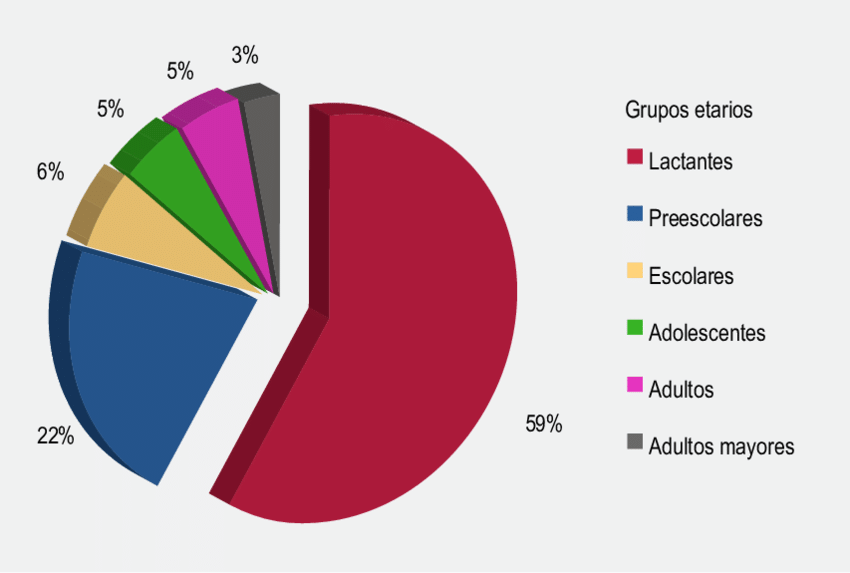
\includegraphics[width=0.8\textwidth]{imagenes/resultados.png}
    \caption{Resultados de exactitud para la clasificación de imágenes.}
    \label{fig:gavali1}  
    \textit{Fuente.} Tomado del trabajo de \cite{zoph2018learning}
\end{figure}

\section{Análisis inferencial}

Para determinar si existen diferencias estadísticamente significativas entre los grupos evaluados, se aplicaron pruebas estadísticas inferenciales.

Se utilizó la prueba \textit{t} de Student para muestras independientes, con un nivel de significancia de $\alpha = 0.05$, para comparar las puntuaciones medias de desarrollo del habla entre Grupo A y Grupo B.

Los resultados obtenidos muestran que no existen diferencias significativas en la edad entre los grupos ($t(38) = -0.68, p = 0.50$), asegurando la comparabilidad de las muestras.

En cuanto a la puntuación en la prueba de habla, se observó una diferencia significativa a favor del Grupo B ($t(38) = -2.14, p = 0.038$), lo que indica un mejor desempeño en este grupo.

Estos resultados sugieren que la implementación de las actividades generadas por IA puede influir positivamente en el desarrollo del habla en niños con Síndrome de Down.

\vspace{0.3cm}
\noindent
\textbf{Nota:} Para realizar estos análisis se utilizó el software estadístico [indicar software, por ejemplo, SPSS, R, Python].

